%\RequirePackage[l2tabu, orthodox]{nag}
\documentclass[12pt]{beamer}
\graphicspath{{Imagenes/}{../Imagenes/}}
\usepackage[utf8]{inputenc}
\usepackage[spanish]{babel}
\usepackage[autostyle,spanish=mexican]{csquotes}
\usepackage{hyperref}
\hypersetup{
  colorlinks=true,
  linkcolor=blue,          % color of internal links (change box color with linkbordercolor)
  citecolor=green,        % color of links to bibliography
  filecolor=magenta,      % color of file links
  urlcolor=cyan,           % color of external links
  linkbordercolor={0 0 1}
}
\usepackage{amsmath}
\usepackage{amsthm}
\usepackage{multicol}
\usepackage{graphicx}
\usepackage{tabulary}
\usepackage{booktabs}
\usepackage{makecell}
\usepackage[outdir=./]{epstopdf}
%\usepackage{epstopdf}
\usepackage{media9}
\usepackage{multimedia}
\usepackage[binary-units=true]{siunitx}
\usepackage{standalone}
\usepackage{longtable}
\usepackage{bigints}
\usepackage{framed}
%\usepackage[font=footnotesize,textfont=it]{caption}
%\usepackage{enumitem}
\usepackage{tikz}
\usepackage{tikz-3dplot}
\tdplotsetmaincoords{70}{120}
\usepackage{silence}
\WarningsOff[catoptions]
% \usepackage{catoptions}
% % before loading circuitikz
% \usepackage{silence}
% \WarningsOff[catoptions]
% \usepackage[siunitx, RPvoltages]{circuitikz}
% \usetikzlibrary{arrows, patterns, shapes, decorations.markings, decorations.pathmorphing}
% \usetikzlibrary{matrix,positioning}
% \tikzstyle{every picture}+=[remember picture,baseline]
\usepackage{color}
\usepackage{alltt}
\usepackage{verbatim}
\usepackage{pdflscape}
\usepackage{pdfpages}
\usepackage{fancyvrb}
%\usepackage{picins}
\usepackage[os=win]{menukeys}
\usepackage{pifont}
\usepackage[sfdefault]{roboto}  %% Option 'sfdefault' only if the base font of the document is to be sans serif
%\usepackage[T1]{fontenc}
\setcounter{secnumdepth}{3}
\setcounter{tocdepth}{3}
\DeclareGraphicsExtensions{.pdf,.png,.jpg}
\renewcommand {\arraystretch}{1.5}
\definecolor{ao}{rgb}{0.0, 0.5, 0.0}
\definecolor{bisque}{rgb}{1.0, 0.89, 0.77}
\definecolor{amber}{rgb}{1.0, 0.75, 0.0}
\definecolor{armygreen}{rgb}{0.29, 0.33, 0.13}
\definecolor{alizarin}{rgb}{0.82, 0.1, 0.26}
\definecolor{cadetblue}{rgb}{0.37, 0.62, 0.63}
\newcommand*{\TitleParbox}[1]{\parbox[c]{6cm}{\raggedright #1}}%
\newcommand{\python}{\texttt{python}}
\newcommand{\textoazul}[1]{\textcolor{blue}{#1}}
\newcommand{\azulfuerte}[1]{\textcolor{blue}{\textbf{#1}}}
\newcommand{\funcionazul}[1]{\textcolor{blue}{\textbf{\texttt{#1}}}}
%\normalfont
\usepackage{ccfonts}% http://ctan.org/pkg/{ccfonts}
\usepackage[T1]{fontenc}% http://ctan.or/pkg/fontenc
\renewcommand{\rmdefault}{cmr}% cmr = Computer Modern Roman
\usefonttheme[onlymath]{serif}
\linespread{1.3}
\newcounter{saveenumi}
\newcommand{\seti}{\setcounter{saveenumi}{\value{enumi}}}
\newcommand{\conti}{\setcounter{enumi}{\value{saveenumi}}}
\newcommand{\tikzmark}[1]{\tikz[remember picture] \node[coordinate] (#1) {#1};}

%reduce el tamaño de letra de la etiqueta equations
\makeatletter
\def\maketag@@@#1{\hbox{\m@th\normalfont\small#1}}
\makeatother

%se usa para la x en itemize
\newcommand{\xmark}{\text{\ding{55}}}

%\AtBeginDocument{\setlength{\tymin}{1em}}


\definecolor{myblue}{rgb}{.8, .8, 1}

\usepackage{amsmath}
\usepackage{empheq}

\newlength\mytemplen
\newsavebox\mytempbox

\makeatletter
\newcommand\mybluebox{%
    \@ifnextchar[%]
       {\@mybluebox}%
       {\@mybluebox[0pt]}}

\def\@mybluebox[#1]{%
    \@ifnextchar[%]
       {\@@mybluebox[#1]}%
       {\@@mybluebox[#1][0pt]}}

\def\@@mybluebox[#1][#2]#3{
    \sbox\mytempbox{#3}%
    \mytemplen\ht\mytempbox
    \advance\mytemplen #1\relax
    \ht\mytempbox\mytemplen
    \mytemplen\dp\mytempbox
    \advance\mytemplen #2\relax
    \dp\mytempbox\mytemplen
    \colorbox{myblue}{\hspace{1em}\usebox{\mytempbox}\hspace{1em}}}

\makeatother

\renewcommand{\labelenumi}{\thesection.\arabic{enumi}}
\renewcommand{\labelenumii}{\thesection.\arabic{enumi}.\arabic{enumii}}

\newcolumntype{L}[1]{>{\raggedright\let\newline\\\arraybackslash\hspace{0pt}}m{#1}}
\newcolumntype{C}[1]{>{\centering\let\newline\\\arraybackslash\hspace{0pt}}m{#1}}
\newcolumntype{R}[1]{>{\raggedleft\let\newline\\\arraybackslash\hspace{0pt}}m{#1}}
%Se usa la plantilla Warsaw modificada con spruce
\mode<presentation>
{
  \usetheme{Warsaw}
  \setbeamertemplate{headline}{}
  \useoutertheme{default}
  %\usecolortheme{beaver}
  \setbeamercovered{invisible}
}
%\AtBeginSection[]
%{
%\begin{frame}<beamer>{Contenido}
%\normalfont\mdseries
%\tableofcontents[currentsection]
%\end{frame}
%}

\setbeamertemplate{section in toc}[sections numbered]
\setbeamertemplate{subsection in toc}[subsections numbered]
\setbeamertemplate{subsection in toc}{\leavevmode\leftskip=3.2em\rlap{\hskip-2em\inserttocsectionnumber.\inserttocsubsectionnumber}\inserttocsubsection\par}
\setbeamercolor{section in toc}{fg=blue}
\setbeamercolor{subsection in toc}{fg=blue}
\setbeamertemplate{navigation symbols}{}
\setbeamercolor{frametitle}{fg=yellow,bg=blue!70!white}
\setbeamercolor{section in head/foot}{bg=gray!30,fg=red}
%\setbeamercolor{section in head}{bg=green,fg=red}
\setbeamercolor{subsection in head/foot}{bg=gray!30,fg=black}
\setbeamercolor{author in head/foot}{bg=gray!30}
\setbeamercolor{date in head/foot}{fg=blue}

%\mode<presentation>
%{
%  \usetheme{Warsaw}
%  \setbeamertemplate{headline}{}
%  %\useoutertheme{infolines}
%  \useoutertheme{default}
%  \setbeamercovered{invisible}
%  % or whatever (possibly just delete it)
%}

\makeatletter
\setbeamertemplate{footline}
{
  \leavevmode%
  \hbox{%
  \begin{beamercolorbox}[wd=.333333\paperwidth,ht=2.25ex,dp=1ex,center]{author in head/foot}%
    \usebeamerfont{author in head/foot} \insertsection
  \end{beamercolorbox}}%
  \begin{beamercolorbox}[wd=.333333\paperwidth,ht=2.25ex,dp=1ex,center]{title in head/foot}%
    \usebeamerfont{title in head/foot} \insertsubsection
  \end{beamercolorbox}%
  \begin{beamercolorbox}[wd=.333333\paperwidth,ht=2.25ex,dp=1ex,right]{date in head/foot}%
    \usebeamerfont{date in head/foot} \textcolor{white}{\insertshortdate{}} \hspace*{2em}
    \textcolor{white}{\insertframenumber{} / \inserttotalframenumber}\hspace*{2ex} 
  \end{beamercolorbox}}%
  \vskip0pt%
\makeatother

%Reduce el espacio entre los items de la TOC
\makeatletter
\patchcmd{\beamer@sectionintoc}{\vskip1.5em}{\vskip0.8em}{}{}
\makeatother
\title{Matemáticas Avanzadas de la Física}
\subtitle{Semestre 2022-1}
\newcommand\RBox[1]{%
  \tikz\node[draw,rounded corners,align=center,] {#1};%
}
\institute{Facultad de Ciencias - UNAM}
\titlegraphic{
\includegraphics[width=2cm]{escudo-facultad-ciencias.jpg}\hspace*{3.75cm}~%
   
\includegraphics[width=2cm]{escudo-unam.jpg}
}
\date{30 de agosto de 2021}
\setbeamertemplate{itemize items}{>>}

\begin{document}
\maketitle
\begin{frame}
\frametitle{Equipo académico}
\begin{center}
\RBox{
M. en C. Gustavo Contreras Mayén \\
\href{mailto:gux7avo@ciencias.unam.mx}{gux7avo@ciencias.unam.mx}
}
\vskip 1cm
\RBox{
M. en C. Abraham Lima Buendía \\
\href{mailto:abraham3081@ciencias.unam.mx}{abraham3081@ciencias.unam.mx}
}
\end{center}
\end{frame}

\section*{Contenido}
\frame{\frametitle{Contenido}\tableofcontents[currentsection, hideallsubsections]}
\fontsize{14}{14}\selectfont
\spanishdecimal{.}

\section{Presentación del curso}
\frame{\frametitle{Contenido}\tableofcontents[currentsection, hideothersubsections]}
\subsection{Objetivos}

\begin{frame}
\frametitle{Objetivos del curso}
En la página de la Facultad, el programa de la asignatura: Matemáticas Avanzadas de la Física se puede consultar \href{http://www.fciencias.unam.mx/asignaturas/610.pdf}{(aquí)}, y contiene los siguientes objetivos:
\end{frame}
\begin{frame}
\frametitle{Objetivos del curso}
En donde el alumno:
\begin{itemize}
\setlength{\itemsep}{0mm}
\item Reconocerá las ideas básicas del análisis de ecuaciones que involucran a funciones de varias variables.
\item Formulará aproximaciones consistentes a soluciones, con el fin de cuantificar los distintos mecanismos de la física que se involucran.
\end{itemize}
\end{frame}
\begin{frame}
\frametitle{Objetivos del curso}
Además:
\begin{itemize}
\setlength{\itemsep}{0mm}
\item Consultará la literatura matemática que sea relevante para los problemas de física.
\item Identificará el papel moderno que juegan las funciones especiales, como auxiliares poderosos en el análisis cualitativo de problemas en varias variables.
\end{itemize}
\end{frame}
\begin{frame}
\frametitle{Objetivo adicional}
También es nuestro objetivo demostrar al alumno que \emph{las funciones especiales y las transformadas integrales} no son solamente un tema matemático, que involucra las ramas de la geometría diferencial, las ecuaciones diferenciales y el análisis matemático.
\end{frame}
\begin{frame}
\frametitle{Objetivo adicional}
Veremos que \emph{son las técnicas de estudio fundamentales} en la electrostática, la electrodinámica, la mecánica cuántica en los límites relativista y no relativista, la dinámica de medios deformables, la hidrodinámica clásica entre otras ramas de la física.
\end{frame}
\begin{frame}
\frametitle{Relevancia de la asignatura}
MAF les brindará un manejo más fluido y consistente para lo que van a cursar en el sexto semestre y los tres semestres que les restan para concluir la carrera.
\\
\bigskip
\pause
Es una asignatura con bastante relevancia para la formación del físico.
\end{frame}

\section{Metodología de enseñanza}
\frame[allowframebreaks]{\tableofcontents[currentsection, hideothersubsections]}
\subsection{Semestre a distancia}

\begin{frame}
\frametitle{Situación en la UNAM}
Aún nos encontramos en contingencia sanitaria por Covid-19, por lo que las autoridades de la UNAM han decidido que el semestre 2022-1 se imparta en modalidad a distancia.
\end{frame}
\begin{frame}
\frametitle{Forma distinta de trabajo}
Continuamos enfrentado el reto de atender actividades síncronas y asíncronas, no solo para el curso de MAF, sino para aquellas actividades que corresponden al sexto semestre.
\end{frame}
\begin{frame}
\frametitle{Trabajo a distancia}
Para este semestre 2022-1 hemos replanteado actividades y el desarrollo del trabajo para la asignatura.
\end{frame}
\begin{frame}
\frametitle{Plataforma de trabajo}
Para este curso utilizaremos la plataforma Moodle, favoreciendo una estandarización con las demás asignaturas que se imparten en la Facultad de Ciencias.
\end{frame}
\begin{frame}
\frametitle{Acceso a Moodle}
Se proporcionarán las credenciales para ingresar a la plataforma en donde encontrarán las actividades de trabajo, materiales de consulta y referencias adicionales para el curso.
\end{frame}
\begin{frame}
\frametitle{Materiales de trabajo}
Se contará con materiales que deberán de revisar: en ellos se discute el tema, se presentan ejemplos, se incluyen ejercicios a cuenta.
\\
\bigskip
La lectura y trabajo con estos materiales es \emph{obligatoria.}
\end{frame}
\begin{frame}
\frametitle{Materiales adicionales}
De manera complementaria se dispondrá de materiales adicionales de consulta, en ellos se hará un revisión en particular de un ejercicio o problema.
\end{frame}
\begin{frame}
\frametitle{Materiales adicionales}
Buscando que el desarrollo se aborde con otro enfoque, pero que complementa lo que hayan revisado en los materiales de trabajo.
\\
\bigskip
Recomendamos mucho que revisen estos materiales adicionales.
\end{frame}
\begin{frame}
\frametitle{Canal de YouTube}
Se han elaborado videos en donde se trabajan ejercicios y ejemplos para los temas.
\\
\bigskip
\pause
Dentro de Moodle se estarán incorporando las ligas para el canal de YouTube, de tal manera que podrán revisar los videos en el momento que ustedes consideren oportuno.
\end{frame}
\begin{frame}
\frametitle{Canal en YouTube}
\begin{figure}[H]
  \centering
  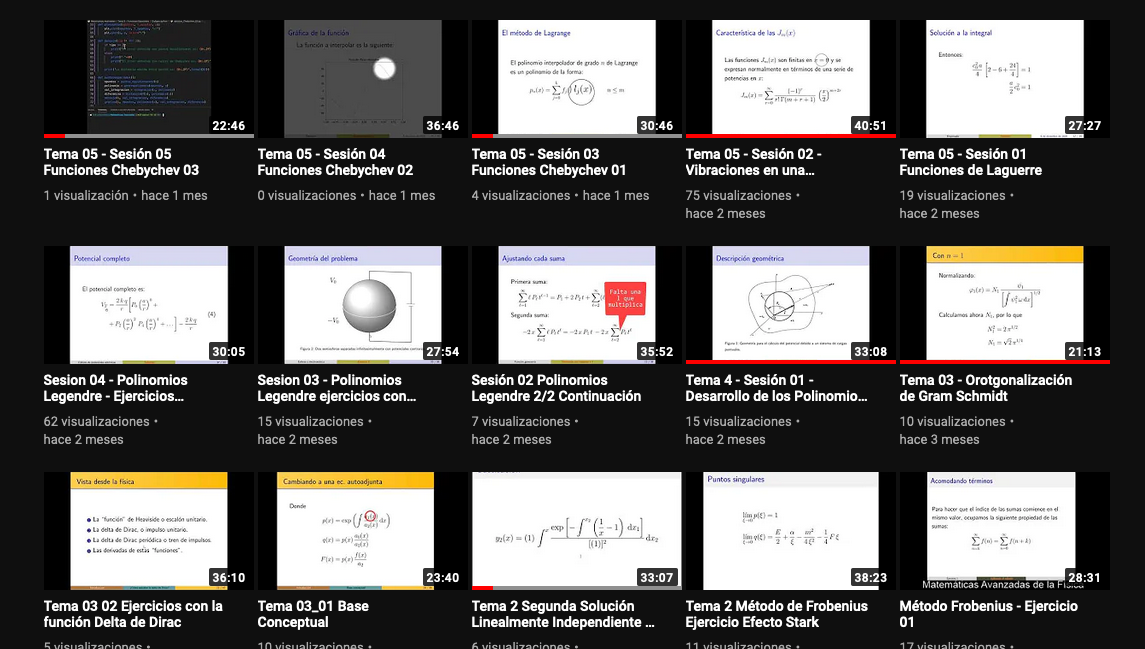
\includegraphics[scale=0.25]{Imagenes/canal_videos.png}
\end{figure}
\end{frame}

\subsection{Formato de trabajo en línea}

\begin{frame}
\frametitle{Formato de trabajo en línea}
Considerando el potencial de la enseñanza a distancia, tendremos un formato de trabajo mixto:
\setbeamercolor{item projected}{bg=blue!70!black,fg=yellow}
\setbeamertemplate{enumerate items}[circle]
\begin{enumerate}[<+->]
\item Con sesiones síncronas en el horario de 3 a 4 pm, que corresponde al horario de la clase.
\item Sesiones asíncronas en donde podrán ingresar a la plataforma Moodle.
\end{enumerate}
\end{frame}
\begin{frame}
\frametitle{Sesiones síncronas}
Se tendrán sesiones de videoconferencia al inicio de cada tema del curso, con la finalidad de presentar:
\setbeamercolor{item projected}{bg=blue!70!black,fg=yellow}
\setbeamertemplate{enumerate items}[circle]
\begin{enumerate}[<+->]
\item Los objetivos.
\item El alcance para ese tema.
\item Indicar las actividades y cronograma de trabajo.
\item Así como el esquema de evaluación para el tema.
\end{enumerate}
\end{frame}
\begin{frame}
\frametitle{Sesiones síncronas}
Las sesiones se llevarán a cabo los días \textcolor{red}{miércoles} y \textcolor{red}{viernes}, en el horario de la asignatura: 3 a 4 pm.
\\
\bigskip
\pause
En algún momento se realizará un ajuste en los días, debido ya sea a días feriados, inicio de un nuevo tema, etc.
\end{frame}
\begin{frame}
\frametitle{Asistencia a la sesiones síncronas}
Es muy importante asistir a las sesiones síncronas, se utilizará el servicio \textcolor{blue}{Zoom} para la videoconferencia.
\\
\bigskip
\pause
Siendo necesario el contar con un equipo de cómputo, una tableta o un teléfono celular.
\begin{figure}
    \centering
    
\includegraphics[scale=0.05]{Logo_Zoom.png}
\end{figure}
\end{frame}
\begin{frame}
\frametitle{Uso de cuenta @ciencias}
Con la finalidad de contar con la mayoría de los servicios en cuanto a TIC que ofrece la UNAM, es necesario utilizar un correo electrónico con el dominio \texttt{@ciencias.unam.mx}
\end{frame}
\begin{frame}
\frametitle{Sesiones asíncronas}
La modalidad de enseñanza a distancia requiere que el alumno realice actividades de manera asíncrona dentro de la plataforma, éstas actividades consistirán en la revisión de materiales de trabajo, lecturas adicionales y videos, consulta de textos complementarios y una serie de ejercicios.
\end{frame}
\begin{frame}
\frametitle{Sesiones asíncronas}
El avance del curso se dará conforme al temario que se revisará en esta presentación, cabe señalar que las actividades (ejercicios y tareas) se deberán de completar en los tiempos señalados, la modalidad a distancia requiere también de un cumplimiento para el alcance de los objetivos.
\end{frame}
{
\setbeamercolor{background canvas}{bg=}
\includepdf[pages=1]{Calendario_Esquema_Trabajo_2022_1.pdf}
}

\subsection{Tiempo para atender el curso}

\begin{frame}
\frametitle{Requerimiento de tiempo}
De manera independiente a la modalidad de trabajo, deben de considerar \enquote{apartar} tiempo para la asignatura, por lo que hacemos la recomendación de que midan su carga académica durante este semestre.
\end{frame}
\begin{frame}
\frametitle{Comunicación constante}
Además de contar con los correos electrónicos, se estará utilizando un canal de Telegram para el envío de mensajes generales, así como para notificaciones, avisos, etc.
\\
\bigskip
\begin{figure}
    \centering
    
\includegraphics[scale=0.15]{Logo_Telegram.png}
\end{figure}
\end{frame}
\begin{frame}
\frametitle{Liga y clave para la videoconferencia}
El envío de la liga y las claves de ingreso a las sesiones de Zoom, se hará por correo, nunca por Telegram.
\\
\bigskip
De esta manera se evita que haya ingresos indebidos a las reuniones.
\end{frame}
\begin{frame}
\frametitle{Material de consulta}
Se contará con diversos materiales de consulta: artículos, capítulos de libros, etc. que estarán disponibles tanto en la plataforma Moodle como en la nube de Drive, por lo que tendrán oportunidad de consultarlos libremente.
\end{frame}

\section{Evaluación}
\frame[allowframebreaks]{\small\tableofcontents[currentsection, hideothersubsections]}
\subsection{Elementos para la calificación.}

\begin{frame}
\frametitle{Elementos para la calificación}
El porcentaje para cada elemento de evaluación es el siguiente:
\begin{itemize}
\setlength{\itemsep}{0mm}
\item Ejercicios semanales: $\mathbf{50\%}$.
\item Exámenes - Tarea: $\mathbf{50\%}$.
\end{itemize}
\end{frame}

\subsection{Ejercicios semanales en clase.}

\begin{frame}
\frametitle{Ejercicios semanales en clase}
En los materiales de trabajo semanales habrá una serie ejercicios que deberán de resolverse, de modo que al concluir la semana, esos ejercicios deberán de entregarse resueltos al siguiente viernes, ocupando para ello la plataforma Moodle.
\end{frame}
\begin{frame}
\frametitle{Muy importante}
Cada ejercicio aporta una parte de la evaluación de cada tema del curso, por lo que recomendamos ampliamente la solución de todos los ejercicios, el número de éstos varía pero contabiliza en la calificación.
\end{frame}
\subsection{Exámenes - Tarea}
\begin{frame}
\frametitle{Exámenes - Tarea}
Habrá un Examen - Tarea por cada tema del curso.
\\
\bigskip
\pause
La entrega de los ejercicios se dará de manera oportuna para que los resuelvan y envíen por la plataforma Moodle.
\end{frame}
\begin{frame}
\frametitle{Exámenes Tarea}
El Examen - Tarea se espera que lo entreguen completo, en caso de que no suceda así, se tomará la respectiva parte proporcional de la calificación obtenida.
\end{frame}
\begin{frame}
\frametitle{De los ejercicios y tareas}
En esta asignatura \emph{se revisa y se evalúa el proceso de resolución de un problema, es decir, será necesario detallar cada paso en la solución}.
\\
\bigskip
\pause
Por lo que deberán de considerar que tanto los ejercicios semanales como los exámenes tendrán que ser resueltos a mano.
\end{frame}
\begin{frame}
\frametitle{¿Cómo entregar los ejercicios y tareas?}
Si cuentan con un escáner, se deberá de digitalizar cada una de las hojas que hayan ocupado en un archivo pdf y enviarlo mediante la plataforma.
\\
\bigskip
\pause
En caso de no contar con un escáner para la digitalización de las soluciones, se podrá enviar un archivo con las imágenes de la solución, tomadas con una tableta o el celular.
\end{frame}
\begin{frame}
\frametitle{De los ejercicios y tareas}
Se les pedirá encarecidamente, ser lo más claros en la escritura, numeración de las hojas, el orden y limpieza en sus soluciones, para que así recibamos un archivo que nos permita evaluar su trabajo.
\end{frame}

\subsection{Consideraciones importantes}

\begin{frame}
\frametitle{Consideraciones importantes}
\begin{itemize}
\setlength{\itemsep}{0mm}
\item No se recibirán ejercicios semanales de manera extemporánea, en Moodle quedarán programada la fecha y horario para el envío, una vez que se llega al tiempo indicado, la plataforma ya no permite el envío.
\item No habrá reposición de exámenes.
\end{itemize}
\end{frame}
\begin{frame}
\frametitle{Ejercicios adicionales}
Para favorecer una mejor calificación en los ejercicios, se presentará un conjunto de ejercicios adicionales en cada tema.
\\
\bigskip
\pause
La solución y entrega de estos ejercicios adicionales es opcional, pero no sustituyen a los ejercicios semanales.
\end{frame}
\begin{frame}
\frametitle{Ejercicios semanales y adicionales}
Los ejercicios semanales son los que conforman el $50\%$ de la calificación.
\\
\bigskip
\pause
Los ejercicios opcionales aportarán hasta un $25\%$ a la evaluación correspondiente a los ejercicios semanales.
\end{frame}
\begin{frame}
\frametitle{Ejemplo de los ejercicios}
\fontsize{12}{12}\selectfont
\begin{table}
\begin{tabular}{l c c c }
Tema & \multicolumn{3}{c}{Ejercicios semanales} \\ \hline
& A resolver & Entregados & Calificación \\
Tema 1 & $15$ & $13$ & $8.66$ \\ \hline
Tema 2 & $17$ & $12$ & $7.05$ \\ \hline
Tema 3 & $15$ & $10$ & $6.66$ \\ \hline
\end{tabular}
\end{table}
\pause
\medskip
Cada ejercicio bien resuelto aporta $1$ punto, en caso de que la solución no sea la correcta y se tenga un avance, se anotará una parte proporcional del punto.
\end{frame}
\begin{frame}
\frametitle{Ejemplo de los ejercicios}
\fontsize{12}{12}\selectfont
\begin{table}
\begin{tabular}{l c c c }
Tema & \multicolumn{3}{c}{Ejercicios opcionales} \\ \hline
& A resolver & Entregados & Calificación \\
Tema 2 & $15$ & $13$ & $8.66$ \\ \hline
Tema 3 & $15$ & $10$ & $6.66$ \\ \hline
\end{tabular}
\end{table}
\pause
\medskip
Los ejercicios opcionales comienzan a partir del Tema 2 y se entregarán de manera semanal; cada ejercicio bien resuelto aporta $1$ punto.
\end{frame}
\begin{frame}
\frametitle{Aportación de los ejercicios opcionales}
De la calificación obtenida por los ejercicios opcionales, se sumará hasta el $25\%$ a la calificación de los ejercicios semanales, esto quiere decir que si el total de los ejercicios opcionales está bien resuelto, se sumarán $2.5$ puntos a la calificación de los ejercicios semanales de cada tema.
\end{frame}  
\begin{frame}[fragile]
\frametitle{Evaluación de ejercicios}
\fontsize{12}{12}\selectfont
\begin{table}
\begin{tabular}{l c c c c}
Tema & Sem. & Opc. & Aportación & Calificación \\ \hline
Tema 2 & $\color{blue}{7.05}$ & $8.66$ & $\color{blue}{2.16}$ & $9.21$ \\ \hline
Tema 3 & $\color{blue}{6.66}$ & $6.66$ & $\color{blue}{1.66}$ & $8.32$ \\ \hline
\end{tabular}
\end{table}
\pause
\medskip
Al final del semestre, se promediará la calificación obtenida de los ejercicios semanales, el resultado representa el $50\%$ de la calificación total del curso.
\end{frame}
\begin{frame}
\frametitle{Consideraciones importantes}
\begin{itemize}
\setlength{\itemsep}{0mm}
\item En caso de que la calificación de un examen - tarea (o de más) sea menor a $6$ (seis), el alumno será candidato para presentar el examen final.
\item Para presentar examen final del curso se requiere que el alumno haya entregado los seis exámenes -  tarea del curso.
\end{itemize}
\end{frame}
\begin{frame}
\frametitle{Consideraciones importantes}
\begin{itemize}
\setlength{\itemsep}{0mm}
\item En caso de no haber entregado alguna tarea semanal de ejercicios y/o no haber presentado un examen del curso, no se tendrá derecho a presentar el examen final, por lo que la calificación final que se asentará en el acta del curso, será \textbf{NP (No presentó)}.
\end{itemize}
\end{frame}
\begin{frame}
\frametitle{Consideraciones importantes}
\begin{itemize}
\setlength{\itemsep}{0mm}
\item En caso de haber presentado al menos un examen y/o haber entregado una tarea semanal de ejercicios, y posteriormente no se tenga registro de otra entrega, se entenderá que abandonaron el curso, por lo que no se tendrá derecho para presentar el examen final, y la calificación que se asentará en el acta del curso, será $\mathbf{5}$ \textbf{(cinco)}.
\end{itemize}
\end{frame}
\begin{frame}
\frametitle{Ejemplo de evaluaciones}
\fontsize{12}{12}\selectfont
\begin{table}
\begin{tabular}{| l | c | c | c | c | c | c | c | c |} \hline
& \multicolumn{2}{c |}{Tema 1} & \multicolumn{2}{c |}{Tema 2} & $\ldots$ & \multicolumn{2}{c |}{Tema 6} & \\ \hline
Alumno & Ex1 & Ej1 & Ex2 & Ej2 & $\ldots$ &  Ex6 & Ej6 & Final \\ \hline
C. López & $8.2$ & $9.0$ & $0$ & $6.3$ & $\ldots$ & $0$ & $0$ & $\mathbf{5}$ \pause \\ \hline 
J. Nieves & $0$ & $0$ & $0$ & $0$ & $\ldots$ & $0$ & $0$ & \textbf{NP} \\ \hline
\end{tabular}
\end{table}
\end{frame}
\begin{frame}
\frametitle{Consideraciones importantes}
\begin{itemize}
\setlength{\itemsep}{0mm}
\item En caso de presentar la primera ronda del examen final y la calificación obtenida sea no aprobatoria ($<6.0$), se puede presentar una segunda y última ronda del examen final.
\item La calificación obtenida en el examen final, es la que se asentará en actas.
\item Si el alumno no presenta el primer examen final, tendrá como calificación final en acta $\mathbf{5}$ \textbf{(cinco)}. 
\end{itemize}
\end{frame}

\section{Temario}
\frame[allowframebreaks]{\small\tableofcontents[currentsection, hideothersubsections]}
\subsection{La física y la geometría}

\begin{frame}
\frametitle{Tema 1 - La física y la geometría}
\setbeamercolor{item projected}{bg=blue!70!black,fg=yellow}
\setbeamertemplate{enumerate items}[circle]
\begin{enumerate}[<+->]
\item Sistemas de coordenadas curvilíneas ortogonales.
\item Operadores diferenciales en coordenadas curvilíneas.
\item Funciones Gamma y Beta.
\end{enumerate}
\end{frame}
\subsection{Primeras técnicas de solución}
\begin{frame}
\frametitle{Tema 2- Primeras técnicas de solución}
\setbeamercolor{item projected}{bg=blue!70!black,fg=yellow}
\setbeamertemplate{enumerate items}[circle]
\begin{enumerate}[<+->]
\item Técnica de separación de variables.
\item Método de Frobenius y remoción de singularidades.
\item Segunda solución linealmente independiente.
\item La delta de Dirac.
\item Momento angular.
\end{enumerate}
\end{frame}
\subsection{Bases completas y ortogonales}
\begin{frame}
\frametitle{Tema 3 - Bases completas y ortogonales}
\setbeamercolor{item projected}{bg=blue!70!black,fg=yellow}
\setbeamertemplate{enumerate items}[circle]
\begin{enumerate}[<+->]
\item Ecuaciones de tipo Sturm-Liouville.
\item Ortogonalización de Gram-Schimdt.
\item Teorema del desarrollo.
\item Función de Green.   
\end{enumerate}
\end{frame}
\subsection{Sep. variables en coordenadas esféricas}
\begin{frame}
\frametitle{Tema 4 - Sep. de variables en coordenadas esféricas}
\framesubtitle{Análisis del átomo de hidrógeno}
\setbeamercolor{item projected}{bg=blue!70!black,fg=yellow}
\setbeamertemplate{enumerate items}[circle]
\begin{enumerate}[<+->]
\item \textcolor{blue}{Parte radial}: Ec. asociada de Laguerre. Ec. ordinaria de Laguerre.
\item \textcolor{blue}{Parte angular}:
\item Armónicos esféricos.
\item Teorema de adición.
\item Ecuación asociada de Legendre. Ecuación ordinaria de Legendre.
\end{enumerate}
\end{frame}
\subsection{Funciones especiales}
\begin{frame}
\frametitle{Tema 5 - Funciones especiales}
\setbeamercolor{item projected}{bg=blue!70!black,fg=yellow}
\setbeamertemplate{enumerate items}[circle]
\begin{enumerate}[<+->]
\item Funciones de Bessel. (Propagación de ondas cilíndricas)
\item Funciones de Hermite. (Oscilador armónico cuántico)
\item Funciones de Chebychev (Interpolación numérica)
\item Funciones de Gegenbauer. 
\item Funciones hipergeométricas: ordinaria y confluente.
\end{enumerate}
\end{frame}
\subsection{Transformadas integrales}
\begin{frame}
\frametitle{Tema 6 - Transformadas integrales}
\setbeamercolor{item projected}{bg=blue!70!black,fg=yellow}
\setbeamertemplate{enumerate items}[circle]
\begin{enumerate}[<+->]
\item Transformada de Fourier.
\item Transformada discreta de Fourier.
\item Transformada rápida de Fourier.
\item Transformada de Laplace.
\end{enumerate}
\end{frame}

\section{Cronograma de trabajo}
\frame{\tableofcontents[currentsection, hideothersubsections]}
\subsection{Calendarización del curso}

\begin{frame}
\frametitle{Calendarización}
A continuación se presenta el cronograma de trabajo para el curso, durante las 16 semanas del semestre se han distribuido los 6 temas.
\end{frame}
{
\setbeamercolor{background canvas}{bg=}
\includepdf[pages=1-6]{Calendario_2022_1.pdf}
}

\section{Fechas importantes}
\frame{\tableofcontents[currentsection, hideothersubsections]}
\subsection{Calendario oficial}

\begin{frame}
\frametitle{Fechas importantes}
%\fontsize{12}{12}\selectfont
\begin{itemize}
\item \textcolor{red}{Lunes 20 de septiembre del 2021. Inicio del semestre 2022-1.}
\item Lunes 1 de noviembre del 2021. Día de asueto.
\item Martes 2 de noviembre del 2021. Día de asueto.
\item Lunes 15 de noviembre del 2021. Día de asueto.
\item \textcolor{blue}{Del Lunes 20 de diciembre al Miércoles 5 de enero de 2022. Período Vacacional de Fin de Año.}
\end{itemize}
\end{frame}
\begin{frame}
\frametitle{Fechas importantes}
%\fontsize{12}{12}\selectfont
\begin{itemize}
\item \textcolor{red}{Viernes 28 de enero de 2022. Termina el semestre 2022-1.}
\item Del lunes 31 de enero al viernes 4 de febrero de 2022. \underline{Primera semana de exámenes}.
\item Del lunes 7 al 11 de febrero del 2022. \underline{Segunda semana de exámenes}.
\end{itemize}
\end{frame}
\begin{frame}
\frametitle{Para ingresar a Moodle}
Se enviará un mensaje por correo electrónico con la clave de acceso a la plataforma Moodle, de tal manera que el registro en la misma y al curso, es de manera personal.
\\
\bigskip
En caso de que consideres algún otro grupo, no será necesario que te registres. %Debiendo realizar el respectivo trámite de baja del grupo $8187$.
\end{frame}
\begin{frame}
\frametitle{Preguntas y respuestas}
Luego de haber revisado la presentación, les pedimos gentilmente realicen las preguntas que consideren necesarias para aclarar cualquiera de los puntos expuestos.
\end{frame}
\end{document}